% Agent–Environment interaction diagram – PPT colour scheme (v3)
% Schematic globe with colours, winking smiling robot
% Compile: xelatex agent_environment_tikz_v3.tex
% Convert: pdf2svg agent_environment_tikz_v3.pdf agent_environment_tikz_v3.svg
\documentclass[border=10pt]{standalone}
\usepackage{fontspec}
\setmainfont{Aptos}[
  Path = /Applications/Microsoft Word.app/Contents/Resources/DFonts/,
  Extension = .ttf,
  UprightFont = Aptos,
  BoldFont = Aptos-Bold,
  ItalicFont = Aptos-Italic,
  BoldItalicFont = Aptos-Bold-Italic,
]
\usepackage{amsmath,amssymb}
\usepackage{tikz}
\usetikzlibrary{arrows.meta, calc}

% PPT colours
\definecolor{accent}{HTML}{CB8044}
\definecolor{fg}{HTML}{E8E8E8}
\definecolor{fgdim}{HTML}{AAAAAA}
% Globe colours (from the original PNG)
\definecolor{land}{HTML}{7BA656}
\definecolor{ocean}{HTML}{5C85A8}

\begin{document}
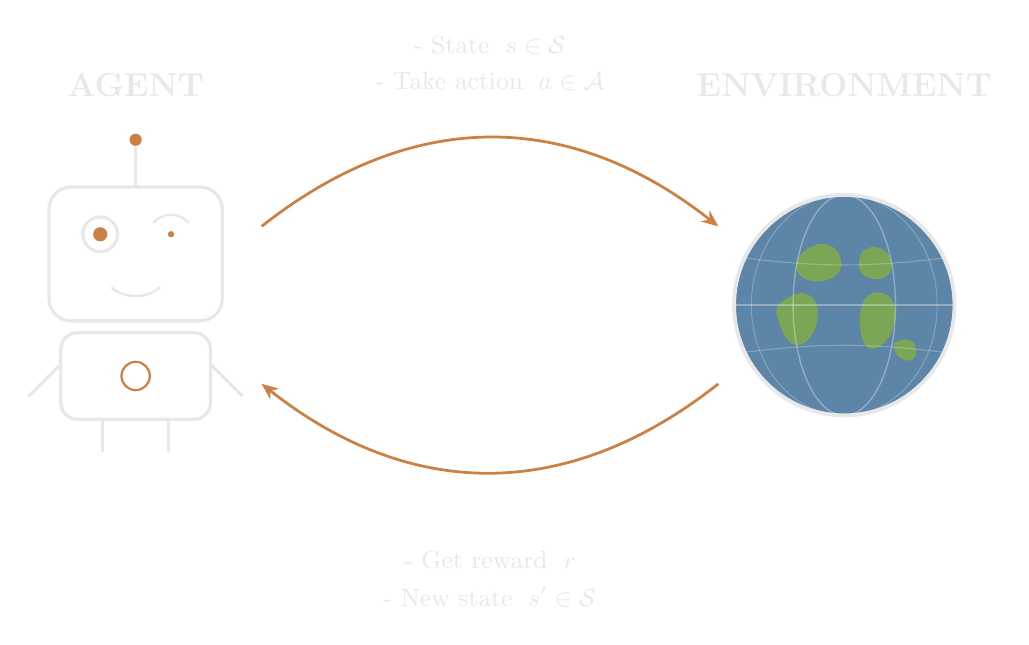
\begin{tikzpicture}[
    >=Stealth,
    curvedarrow/.style={
        accent,
        line width=1pt,
        -{Stealth[length=6pt, width=5pt]},
    },
]

% =============================================
% AGENT – Wireframe robot with smile and wink
% =============================================
\begin{scope}[shift={(0,0)}, fg, line width=1.2pt, line cap=round, line join=round]
  % Head
  \draw[rounded corners=8pt] (-1.1,0.3) rectangle (1.1,2.0);
  % Antenna stem
  \draw (0,2.0) -- (0,2.5);
  % Antenna tip
  \fill[accent] (0,2.6) circle (2.2pt);
  % Left eye – open
  \draw (-.45,1.4) circle (0.22);
  \fill[accent] (-.45,1.4) circle (0.09);
  % Right eye – winking (closed arc above eye level)
  \draw[line width=0.9pt] (0.23,1.55) .. controls (0.35,1.68) and (0.55,1.68) .. (0.67,1.55);
  \fill[accent] (0.45,1.4) circle (0.04);
  % Mouth – smile
  \draw[line width=0.9pt] (-0.3,0.72) .. controls (-0.15,0.58) and (0.15,0.58) .. (0.3,0.72);
  % Body
  \draw[rounded corners=6pt] (-0.95,-0.95) rectangle (0.95,0.15);
  % Body accent circle
  \draw[accent, line width=0.8pt] (0,-0.4) circle (0.18);
  % Arms
  \draw (-0.95,-0.25) -- (-1.35,-0.65);
  \draw (0.95,-0.25) -- (1.35,-0.65);
  % Legs
  \draw (-0.42,-0.95) -- (-0.42,-1.35);
  \draw (0.42,-0.95) -- (0.42,-1.35);
\end{scope}

% Agent label
\node[fg, font=\fontsize{12}{14}\selectfont\bfseries] at (0,3.3) {AGENT};

% =============================================
% ENVIRONMENT – Schematic globe with colours
% =============================================
\begin{scope}[shift={(9,0.5)}]
  % Ocean fill
  \fill[ocean] (0,0) circle (1.4);

  % Land mass blobs (stylised, organic)
  \fill[land] (-0.55,0.65)
    .. controls (-0.35,0.85) and (-0.1,0.8) .. (-0.05,0.6)
    .. controls (0.0,0.4) and (-0.15,0.3) .. (-0.35,0.3)
    .. controls (-0.55,0.3) and (-0.7,0.45) .. (-0.55,0.65);
  \fill[land] (0.25,0.7)
    .. controls (0.4,0.8) and (0.6,0.7) .. (0.6,0.5)
    .. controls (0.6,0.35) and (0.45,0.3) .. (0.3,0.35)
    .. controls (0.15,0.4) and (0.15,0.6) .. (0.25,0.7);
  \fill[land] (0.35,0.15)
    .. controls (0.5,0.2) and (0.65,0.1) .. (0.65,-0.1)
    .. controls (0.65,-0.3) and (0.55,-0.5) .. (0.4,-0.55)
    .. controls (0.25,-0.6) and (0.2,-0.4) .. (0.2,-0.2)
    .. controls (0.2,0.0) and (0.25,0.1) .. (0.35,0.15);
  \fill[land] (-0.7,0.1)
    .. controls (-0.55,0.2) and (-0.4,0.15) .. (-0.35,0.0)
    .. controls (-0.3,-0.2) and (-0.4,-0.45) .. (-0.55,-0.5)
    .. controls (-0.7,-0.55) and (-0.8,-0.35) .. (-0.85,-0.15)
    .. controls (-0.9,0.0) and (-0.8,0.05) .. (-0.7,0.1);
  \fill[land] (0.7,-0.45)
    .. controls (0.85,-0.4) and (0.95,-0.5) .. (0.9,-0.65)
    .. controls (0.85,-0.75) and (0.7,-0.7) .. (0.65,-0.6)
    .. controls (0.6,-0.5) and (0.62,-0.47) .. (0.7,-0.45);

  % Schematic grid lines (on top of colours)
  % Vertical meridian (central)
  \draw[fg, line width=0.5pt, opacity=0.4] (0,-1.4) arc[start angle=-90, end angle=90, x radius=0.65, y radius=1.4];
  \draw[fg, line width=0.5pt, opacity=0.4] (0,1.4) arc[start angle=90, end angle=270, x radius=0.65, y radius=1.4];
  % Wider meridian
  \draw[fg, line width=0.35pt, opacity=0.3] (0,-1.4) arc[start angle=-90, end angle=90, x radius=1.18, y radius=1.4];
  \draw[fg, line width=0.35pt, opacity=0.3] (0,1.4) arc[start angle=90, end angle=270, x radius=1.18, y radius=1.4];
  % Equator
  \draw[fg, line width=0.5pt, opacity=0.4] (-1.4,0) -- (1.4,0);
  % Latitude lines
  \draw[fg, line width=0.4pt, opacity=0.3] (-1.28,0.6) .. controls (-0.3,0.48) and (0.3,0.48) .. (1.28,0.6);
  \draw[fg, line width=0.4pt, opacity=0.3] (-1.28,-0.6) .. controls (-0.3,-0.48) and (0.3,-0.48) .. (1.28,-0.6);

  % Globe outline
  \draw[fg, line width=1.4pt] (0,0) circle (1.4);
\end{scope}

% Environment label
\node[fg, font=\fontsize{12}{14}\selectfont\bfseries] at (9,3.3) {ENVIRONMENT};

% =============================================
% TOP ARROW: Agent -> Environment
% =============================================
\draw[curvedarrow]
    (1.6,1.5) .. controls (3.5,3.0) and (5.5,3.0) .. (7.4,1.5);

% Top labels – placed above the arrow arc
\node[fg, font=\fontsize{9}{11}\selectfont, anchor=south] at (4.5,3.55) {%
  - State\; $s \in \mathcal{S}$%
};
\node[fg, font=\fontsize{9}{11}\selectfont, anchor=south] at (4.5,3.1) {%
  - Take action\; $a \in \mathcal{A}$%
};

% =============================================
% BOTTOM ARROW: Environment -> Agent
% =============================================
\draw[curvedarrow]
    (7.4,-0.5) .. controls (5.5,-2.0) and (3.5,-2.0) .. (1.6,-0.5);

% Bottom labels – placed below the arrow arc
\node[fg, font=\fontsize{9}{11}\selectfont, anchor=north] at (4.5,-2.5) {%
  - Get reward\; $r$%
};
\node[fg, font=\fontsize{9}{11}\selectfont, anchor=north] at (4.5,-2.95) {%
  - New state\; $s' \in \mathcal{S}$%
};

\end{tikzpicture}
\end{document}
